\documentclass{article}
\usepackage{fancyhdr}
\usepackage{amsthm}
\usepackage{etoolbox}
\usepackage{verbatim}
\usepackage{enumerate}
\usepackage{amsmath}
\usepackage{algorithmicx}
\usepackage{algorithm}
\usepackage{algpseudocode}
\usepackage{tikz}


	
\pagestyle{fancy}
\title{Chapter 12}
\author{Michelle Bodnar, Andrew Lohr}

\newcounter{curnum}
\setcounter{curnum}{0}

\newtheorem{th1}{Exercise}
\newcommand{\calH}{\mathcal{H}}
\newcommand{\calX}{\mathcal{X}}
\newcommand{\calA}{\mathcal{A}}
\newcommand{\calY}{\mathcal{Y}}

\begin{document}
\maketitle

\noindent\textbf{ Exercise 12.1-1} \\
Anytime that a node has a single child, treat it as the right child, with the left child being NIL

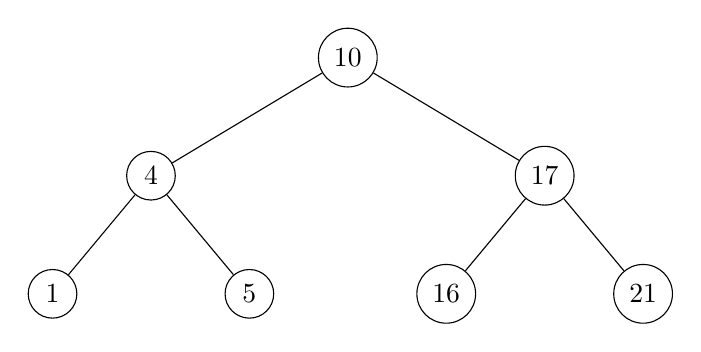
\begin{tikzpicture}[level/.style={sibling distance=50mm/#1}]
\node [circle,draw] (z){10}
  child {node [circle,draw] (a) {4}
    child {node [circle,draw] (b) {1}
      }
    child {node [circle,draw] (g) {5}
  }
  }
  child {node [circle,draw] (a) {17}
    child {node [circle,draw] (b) {16}
	}
    child {node [circle,draw] (g) {21}
  }
        };
\end{tikzpicture}

\begin{tikzpicture}[level/.style={sibling distance=50mm/#1}]
\node [circle,draw] (z){10}
  child {node [circle,draw] (a) {4}
    child {node [circle,draw] (b) {1}
      }
    child {node [circle,draw] (g) {5}
  }
  }
  child {node [circle,draw] (a) {16}
    child {node [circle,draw] (b) {17}
    child {node [circle,draw] (g) {21}
  }}
        };
\end{tikzpicture}

\begin{tikzpicture}[level/.style={sibling distance=50mm/#1}]
\node [circle,draw] (z){5}
  child {node [circle,draw] (a) {1}
    child {node [circle,draw] (g) {4}
  }
  }
  child {node[circle,draw] (y) {10}
  child {node [circle,draw] (a) {16}
    child {node [circle,draw] (b) {17}
    child {node [circle,draw] (g) {21}
  }}}
        };
\end{tikzpicture}

\begin{tikzpicture}[level/.style={sibling distance=50mm/#1}]
\node [circle,draw] (z){4}
  child {node [circle,draw] (a) {1}
  }
   child {node[circle,draw] (x) {5}
  child {node[circle,draw] (y) {10}
  child {node [circle,draw] (t) {16}
    child {node [circle,draw] (b) {17}
    child {node [circle,draw] (g) {21}
  }}}} };
\end{tikzpicture}

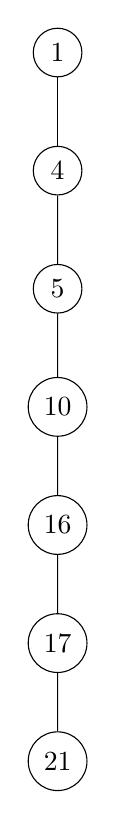
\begin{tikzpicture}[level/.style={sibling distance=50mm/#1}]
\node [circle,draw] (z){1}
  child {node [circle,draw] (x) {4}
   child {node[circle,draw] (t) {5}
  child {node[circle,draw] (y) {10}
  child {node [circle,draw] (a) {16}
    child {node [circle,draw] (b) {17}
    child {node [circle,draw] (g) {21}
  }}}}}
        };
\end{tikzpicture}

\noindent\textbf{ Exercise 12.1-3} \\
Our solution to exercise 10.4-5 solves this problem.\\

\noindent\textbf{ Exercise 12.1-5} \\
Suppose to a contradiction that we could build a bst in worst case time $o(n\lg(n))$. Then, to sort, we would just construct the BST and then read off the elements in an inorder traversal. This second step can be done in time $\Theta(n)$ by Theorem 12.1. Also, an inorder traversal must be in sorted order because the elements in the left subtree are all those that are smaller than the current element, and they all get printed out before the current element, and the elements of the right subtree are all those elements that are larger and they get printed out  after the current element. This would allow us to sort in time $o(n\lg(n))$ a contradiction\\


\noindent\textbf{ Exercise 12.2-1} \\
option $c$ could not be the sequence of nodes explored because we take the left child from the 911 node, and yet somehow manage to get to the 912 node which cannot belong the left subtree of 911 because it is greater. Option $e$ is also impossible because we take the right subtree on the 347 node and yet later come across the 299 node.\\

\noindent\textbf{ Exercise 12.2-3} \\
\begin{algorithm}
\caption TREE-PREDECESSOR(x)
\begin{algorithmic}
\If{$x.left \neq NIL$}
\State \Return TREE-MAXIMUM(x.left)
\EndIf
\State $y = x.p$
\While{$y\neq NIL$ and $x==y.left$}
\State $x=y$
\State $y=  y.p$
\EndWhile
\State\Return $y$
\end{algorithmic}
\end{algorithm}

\noindent\textbf{ Exercise 12.2-5} \\
Suppose the node $x$ has two children. Then it's successor is the minimum element of the BST rooted at $x.right$. If it had a left child then it wouldn't be the minimum element. So, it must not have a left child. Similarly, the predecessor must be the maximum element of the left subtree, so cannot have a right child.\\

\noindent\textbf{ Exercise 12.2-7} \\
To show this bound on the runtime, we will show that using this procedure, we traverse each edge twice. This will suffice because the number of edges in a tree is one less than the number of vertices.

Consider a vertex of a BST, say $x$. Then, we have that the edge between $x.p$ and $x$ gets used when successor is called on $x.p$ and gets used again when it is called on the largest element in the subtree rooted at $x$. Since these are the only two times that that edge can be used, apart from the initial finding of tree minimum. We have that the runtime is $O(n)$. We trivially get the runtime is $\Omega(n)$ because that is the size of the output.

\noindent\textbf{ Exercise 12.2-9} \\
If $x = y.left$ then calling successor on $x$ will result in no iterations of the while loop, and so will return $y$. Similarly, if $x =y.right$, the while loop for calling predecessor(see exercise 3) will be run no times, and so $y$ will be returned. Then, it is just a matter of recognizing what the problem asks to show is exactly that y  is either predecessor(x) or successor(x).

\noindent\textbf{ Exercise 12.3-1} \\


\end{document} 